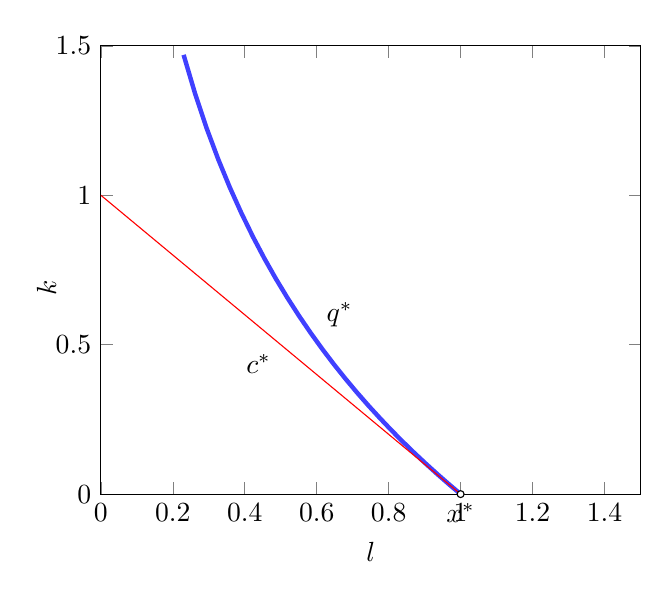
\begin{tikzpicture}
\begin{axis}[
	xmin=0,xmax=1.5,ymin=0,ymax=1.5,
	xlabel style={below},xlabel=$l$,
	ylabel style={left},ylabel=$k$,
	extra x ticks={1},
	extra x tick labels={{$x^*$}}]
\addplot[domain=0.23:1,draw=blue!75,ultra thick] {-ln(x)};
\addplot[red,domain=0:1] {1-x};
\addplot[only marks,forget plot,black,mark options={mark size=1.25pt,fill=white},mark=*] coordinates {(1,0)};
\node[right] at (axis cs:0.6,0.6) {$q^*$};
\node[below left] at (axis cs:0.5,0.5) {$c^*$};
\end{axis}
\end{tikzpicture}
